%%%%%%%%%%%%%%%%%%%%%%%%%%%%%%%% COMMENT THIS TO COMPILE main.tex %%%%%%%%%%%%%%%%%%%%%%%%%%%%%%%%
%\documentclass[a4paper,12pt]{report}
\usepackage[english]{babel}
\usepackage[left=2cm,right=2cm,top=2cm,bottom=2cm]{geometry}
%\usepackage{mathtools}
\usepackage{amsthm}     % for definitions and theorems
\usepackage[many]{tcolorbox}    % boxes around definitions and theorems
%\usepackage{amsmath}
%\usepackage{nccmath}
\usepackage{amssymb}    % \ltimes
\usepackage{etoolbox}   % for start of Chapter
%\usepackage{amsfonts}
\usepackage{physics}    % for all Physics related
\usepackage{dsfont}     % for the identity matrix symbol \1
%\usepackage{mathrsfs}

\usepackage{titling}
\usepackage{indentfirst}

\usepackage{bm}
\usepackage[dvipsnames]{xcolor}
\usepackage{cancel}

\usepackage{xurl}
\usepackage[colorlinks=true]{hyperref}

\usepackage{float}
\usepackage{graphicx}
\usepackage{subcaption}
%\usepackage{tikz}

\usepackage{ctable}     % tabelas
\renewcommand{\P}{\phantom{+}}  % empty space to indent things
\usepackage{multirow}
\usepackage{tabulary}

%%%%%%%%%%%%%%%%%%%%%%%%%%%%%%%%%%%%%%%%%%%%%%%%%%%

\newcommand{\eps}{\epsilon}
\newcommand{\vphi}{\varphi}
\newcommand{\cte}{\text{cte}}

\newcommand{\N}{{\mathbb{N}}}
\newcommand{\Z}{{\mathbb{Z}}}
%\newcommand{\Q}{{\mathbb{Q}}}
\newcommand{\C}{{\mathbb{C}}}
\renewcommand{\S}{{\hat{S}}}
%\renewcommand{\H}{\s{H}}

\renewcommand{\a}{{\vb{a}}}
\renewcommand{\b}{{\vb{b}}}
\renewcommand{\d}{{\dagger}}
\newcommand{\up}{{\uparrow}}
\newcommand{\down}{{\downarrow}}
\newcommand{\hc}{{\text{h.c.}}}

\newcommand{\ihat}{\bm{\hat{\imath}}}
\newcommand{\jhat}{\bm{\hat{\jmath}}}
\newcommand{\khat}{\bm{\hat{k}}}

\newcommand{\0}{{\vb{0}}}
\newcommand{\1}{\mathds{1}}
\newcommand{\E}{{\vb{E}}}
\newcommand{\B}{{\vb{B}}}
\renewcommand{\u}{{\vb{u}}}
\renewcommand{\v}{{\vb{v}}}
\renewcommand{\r}{{\vb{r}}}
\newcommand{\R}{{\vb{R}}}
\newcommand{\Q}{{\vb{Q}}}
\newcommand{\G}{{\vb{G}}}
\newcommand{\g}{{\vb{g}}}
\renewcommand{\k}{{\vb{k}}}
\newcommand{\K}{{\vb{K}}}
\newcommand{\p}{{\vb{p}}}
\newcommand{\q}{{\vb{q}}}
\newcommand{\F}{{\vb{F}}}
\renewcommand{\t}{{\vb{t}}}
\newcommand{\vtau}{{\bm{\tau}}}
\newcommand{\vdelta}{{\bm{\delta}}}

% COLORED SYMMETRY ELEMENTS
\newcommand{\Ct}{{\textcolor{Cyan}{C_3}}}
\newcommand{\Ctn}[1]{{\textcolor{Cyan}{C_3^{\textcolor{black}{#1}}}}}
\newcommand{\Cs}{{\textcolor{ForestGreen}{C_6}}}
\newcommand{\Csn}[1]{{\textcolor{ForestGreen}{C_6^{\textcolor{black}{#1}}}}}
\newcommand{\sd}{{\textcolor{RoyalBlue}{\sigma_d}}}
\newcommand{\sdn}[1]{{\textcolor{RoyalBlue}{\sigma_d^{\textcolor{black}{#1}}}}}
\newcommand{\sdp}{{\textcolor{RoyalBlue}{\sigma_d'}}}
\newcommand{\sdpp}{{\textcolor{RoyalBlue}{\sigma_d''}}}
\newcommand{\sv}{{\textcolor{Orange}{\sigma_v}}}
\newcommand{\svn}[1]{{\textcolor{Orange}{\sigma_v^{\textcolor{black}{#1}}}}}
\newcommand{\svp}{{\textcolor{Orange}{\sigma_v'}}}
\newcommand{\svpp}{{\textcolor{Orange}{\sigma_v''}}}

\newcommand{\s}{\sigma}
%\newcommand{\prodint}[2]{\left\langle #1 , #2 \right\rangle}
\newcommand{\cc}[1]{\overline{#1}}
\newcommand{\Eval}[3]{\eval{\left( #1 \right)}_{#2}^{#3}}
\newcommand{\sg}[2]{\{ #1 \mid #2 \}}

\newcommand{\unit}[1]{\; \mathrm{#1}}

\newcommand{\n}{\medskip}
\newcommand{\e}{\quad \mathrm{and} \quad}
\newcommand{\ou}{\quad \mathrm{or} \quad}
\newcommand{\virg}{\, , \;}
\newcommand{\ptodo}{\forall \,}
\renewcommand{\implies}{\; \Rightarrow \;}
%\newcommand{\eqname}[1]{\tag*{#1}} % Tag equation with name

\setlength{\droptitle}{-7em}

\makeatletter
\patchcmd{\chapter}{\if@openright\cleardoublepage\else\clearpage\fi}{}{}{}  % start 'Chapter' at the same page. needs package etoolbox
\makeatother

%% Theorems, definitions, proofs
\theoremstyle{definition}

\newtheorem{definition}{Definition}[section]
\tcolorboxenvironment{definition}{
  colback=blue!5!white,
  boxrule=0pt,
  boxsep=1pt,
  left=2pt,right=2pt,top=2pt,bottom=2pt,
  oversize=2pt,
  sharp corners,
  before skip=\topsep,
  after skip=\topsep,
}

\newtheorem{theorem}{Theorem}[section]
\tcolorboxenvironment{theorem}{
  colback=blue!5!white,
  boxrule=0pt,
  boxsep=1pt,
  left=2pt,right=2pt,top=2pt,bottom=2pt,
  oversize=2pt,
  sharp corners,
  before skip=\topsep,
  after skip=\topsep,
}

%\begin{document}
%%%%%%%%%%%%%%%%%%%%%%%%%%%%%%%% COMMENT THIS TO COMPILE main.tex %%%%%%%%%%%%%%%%%%%%%%%%%%%%%%%%


%%%%%%%%%%%%%%%%%%%%%%%%%%%%%%%%%%%%%%%%%%%%%%%%%%%%%%%%%%%%%%%%%%%%%%%%%%%%%%%%%%%%%%%%%%%%%%%%%%
\chapter{Topological heavy fermion} \label{ch:topoheavyfermion}
%%%%%%%%%%%%%%%%%%%%%%%%%%%%%%%%%%%%%%%%%%%%%%%%%%%%%%%%%%%%%%%%%%%%%%%%%%%%%%%%%%%%%%%%%%%%%%%%%%

The representations and Elementary Band Representations (EBRs) for a given (magnetic) space group, such as \( P6'2'2 \), can be conveniently obtained from the Bilbao Crystallographic Server \cite{bilbao_1, bilbao_2}.

\begin{table}[H]
\caption{Character table of irreps at high symmetry momenta in magnetic space group $P6'2'2$.}
\centering
\begin{tabular} { c c c c | c c c | c c c }
\cline{1-10}
$\P$ & $\P \Gamma_1$ & $\P \Gamma_2$ & $\P \Gamma_3$ & $\P$ & $\P M_1$ & $\P M_2$ & $\P$ & $\P K_1$ & $\P K_2K_3$ \\
\cline{1-10}
$E$ & $\P1$ & $\P1$ & $\P2$ & $\P E$ & $\P1$ & $\P1$ & $\P E$ & $\P1$ & $\P2$ \\
$2 C_3$ & $\P1$ & $\P1$ & $ -1$ & $\P C_2'$ & $\P1$ & $ -1$ & $\P C_3$ & $\P1$ & $ -1$ \\
$3 C_2'$ & $\P1$ & $ -1$ & $\P0$ & $\P$ & $\P$ & $\P$ & $\P C_3^{-1}$ & $\P1$ & $-1$ \\
\cline{1-10}
\end{tabular}
\label{tab:P6'2'2}
\end{table}

\begin{table}[H]
\footnotesize
\caption{Elementary band representations of the magnetic space group $P6'2'2$.}
\centering
\begin{tabular}{|c|c|c|c|c|c|c|c|c|}
\hline
Wyckoff & \multicolumn{3}{c|}{$1a$} & \multicolumn{3}{c|}{$2c$} & \multicolumn{2}{c|}{$3f$} \\
\cline{1-9}
Site sym. & \multicolumn{3}{c|}{$6'2'2$, $32$} & \multicolumn{3}{c|}{$32$, $32$} & \multicolumn{2}{c|}{$2'2'2$, $2$} \\
\cline{1-9}
EBR & $G_{A_1}^{1a}(1)$ & $G_{A_2}^{1a}(1)$ & $G_{E}^{1a}(2)$ & $G_{A_1}^{2c}(2)$ & $G_{A_2}^{2c}(2)$ & $G_{E}^{2c}(4)$   & $G_{A}^{3f}(3)$ & $G_{B}^{3f}(3)$ \\
\hline
$\Gamma$ & $\Gamma_1$ & $\Gamma_2$ & $\Gamma_3$ & $2\Gamma_1$ & $2\Gamma_2$ & $2\Gamma_3$ & $\Gamma_1+\Gamma_3$ & $\Gamma_2+\Gamma_3$ \\
\hline
$K$ & $K_1$ & $K_1$ & $K_2 K_3$ & $K_2 K_3$ & $K_2 K_3$ & $2K_1 + K_2 K_3$ & $K_1+K_2 K_3$ & $K_1+K_2 K_3$ \\
\hline
$M$ & $M_1$ & $M_2$ & $M_1+M_2$ & $2M_1$ & $2M_2$ & $2M_1+2M_2$ & $2M_1+M_2$ & $M_1+2M_2$ \\
\hline
\end{tabular}
\label{tab:matbg-irreps}
\end{table}

As demonstrated in \cite{all_magic_angles}, incorporating the emergent particle-hole symmetry within the One Valley BM model ensures that the middle two flat bands in each valley align with the irreducible co-representations (irreps):
\begin{equation} \label{eq:matbg-irreps}
\Gamma_1(1) \oplus \Gamma_2(1); \; M_1(1) \oplus M_2(1); \; K_2 K_3(2),
\end{equation}
associated with the magnetic space group \( P6'2'2 \). The characters for each of these irreps, referenced in Equation \ref{eq:matbg-irreps}, are presented in Table \ref{tab:P6'2'2}.


By comparing the irreps in Equation \ref{eq:matbg-irreps} with the EBRs in Table \ref{tab:matbg-irreps}, we observe that the irreps in Equation \ref{eq:matbg-irreps} cannot be expressed as a direct sum of the local orbitals listed in Table \ref{tab:matbg-irreps}. In fact, if we permit negative coefficients, the irreps can only be expressed as the linear combination \( G_{A_1}^{2c} + G_{A_2}^{1a} - G_{A_1}^{1a} \). The presence of a negative coefficient indicates that the two flat bands must host at least a fragile topological phase \cite{FragileTopology_Po2018}, leading to a Wannier obstruction.

To resolve this Wannier obstruction, we incorporate the nearest higher-energy bands, which are characterized by the \(\Gamma_3\) irrep at the \(\Gamma_M\) point \cite{topoheavyfermion2022}. These higher-energy bands hybridize with the two middle bands, allowing us to isolate the trivial bands. These trivial bands form the band representation:
\begin{equation} \label{eq:trivial-irreps}
G_E^{1a}(2) = [E]_{1a} \uparrow G: \quad \Gamma_3(2); \; M_1(1) \oplus M_2(1); \; K_2 K_3(2),
\end{equation}
where \([E]_{1a}\) corresponds to \(p_x \pm i p_y\)-like orbitals at the \(1a\) Wyckoff position.

We ``borrow'' a $\Gamma_3$ irrep from these higher-energy bands to replace the $\Gamma_1 \oplus \Gamma_2$ states. The resulting irreps $\Gamma_3$, $M_1 \oplus M_2$, $K_2 K_3$ are consistent with $p_x \pm i p_y$ orbitals on a triangular lattice. To model this, Gaussian Wannier functions (WFs) that transform as $p_x \pm i p_y$ under the crystal symmetries are introduced.

Using the maximal localization procedure \cite{maxlocalWFs_marzari2012, wannier90}, we find that these WFs are highly localized, supported by flat band states away from $\Gamma_M$, and by low-energy states near $\Gamma_M$. However, to fully account for the superconducting properties, it is crucial to include the remaining states. To achieve this, we define projectors $\bP$ (onto the WFs) and $\I$ (onto the lowest six bands per spin-valley), and decompose the BM Hamiltonian $H_\text{BM}$ into the following components:
\begin{equation} \label{eq:projected_hamiltonians_WFs_PQ}
H^{(f)} = \bP H_\text{BM} \bP, \quad H^{(c)} = \bQ H_\text{BM} \bQ, \quad H^{(fc)} = \bP H_\text{BM} \bQ, \quad H^{(cf)} = H^{(fc)\dagger},
\end{equation}
where $\bQ = \I - \bP$. Since the coupling between WFs is extremely weak, the approximation $H^{(f)} \approx 0$ proves to be highly accurate.

The two states in $\bP$ form $\Gamma_3$ at $\Gamma_M$, while the four states in $\bQ$ form $\Gamma_3 \oplus \Gamma_1 \oplus \Gamma_2$. The remaining Hamiltonian $H^{(c)}$ in valley $\eta$ is expressed as:
\begin{equation} \label{eq:H(c)_topoheavyfermion}
H^{(c, \eta)}(\k) =
\begin{pmatrix}
0_{2\times 2} & v_* (\eta k_x \sigma_0 + i k_y \sigma_z) \\
v_* (\eta k_x \sigma_0 - i k_y \sigma_z) & M \sigma_x
\end{pmatrix}.
\end{equation}

The coupling $H^{(fc)}$ takes the form:
\begin{equation} \label{eq:H(fc)_topoheavyfermion}
H^{(fc, \eta)}(\k) =
\begin{pmatrix}
\gamma \sigma_0 + v'_* (\eta k_x \sigma_x + k_y \sigma_y) & 0_{2\times 2}
\end{pmatrix},
\end{equation}
which introduces a gap in $H^{(c, \eta)}$, establishing the flat band topology of the BM model.

Using standard parameters for MATBG, this mapping provides the parameter values:
\begin{equation} \label{eq:paramaters_topoheavyfermion}
v^\star = -4.303 \, \text{eV} \cdot \AA, \quad M = 3.697 \, \text{meV}, \quad \gamma = -24.75 \, \text{meV}, \quad v'^\star = 1.622 \, \text{eV} \cdot \AA.
\end{equation}

By diagonalizing the resulting 6-band model for the valley $\eta = +$, constructed from the Hamiltonians $H^{(c,\eta)}$ and $H^{(fc,\eta)}$, we obtain the results shown in Figure \ref{fig:thf-exploration}. We analyze the cases where certain parameters are set to zero to study the model's behavior.

\begin{figure}[H]
\centering
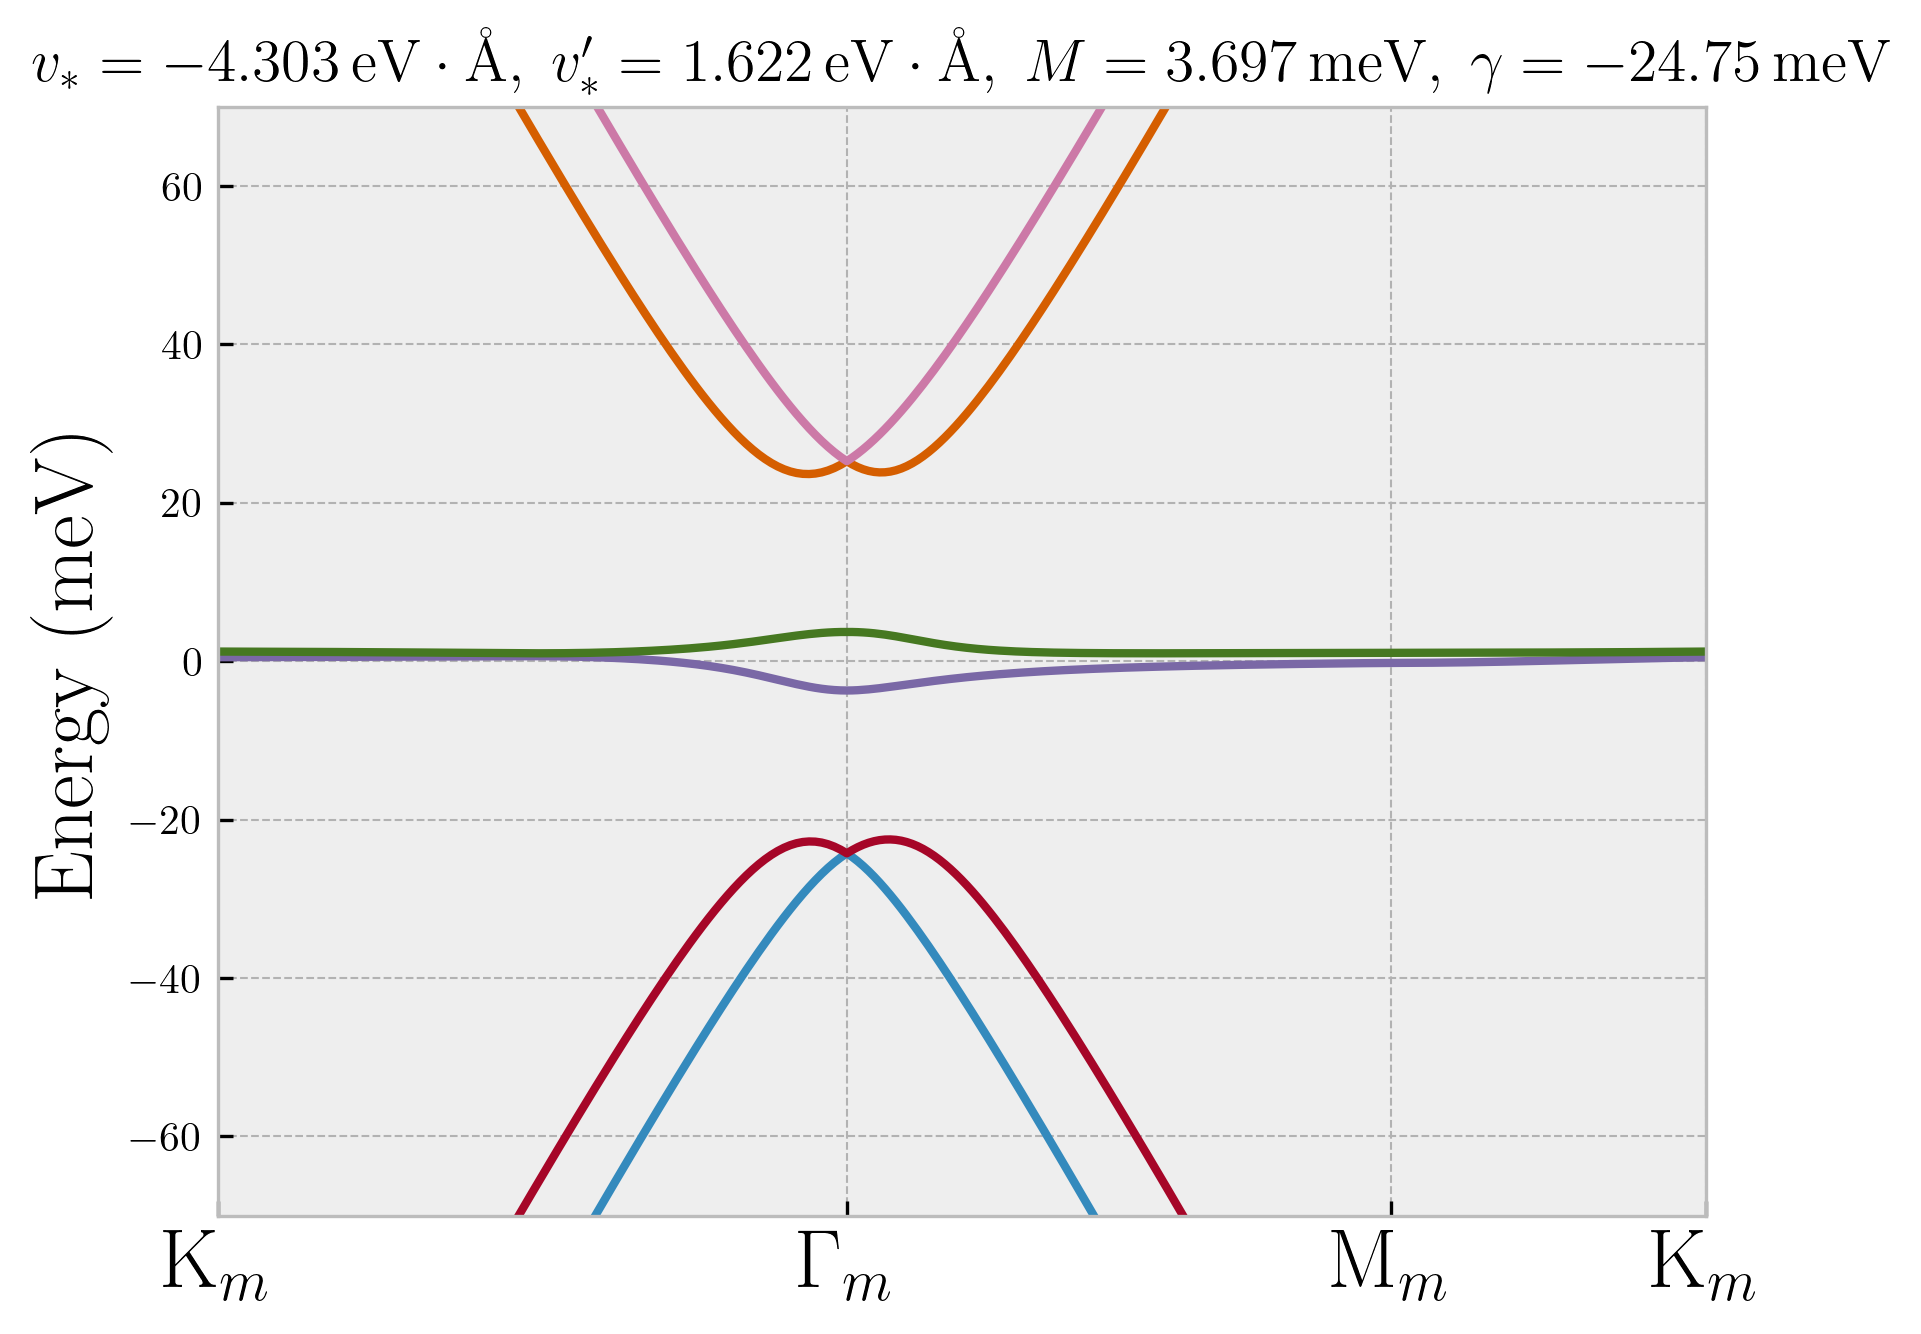
\includegraphics[height=0.25\linewidth]{fig/thf-correct_params.png}
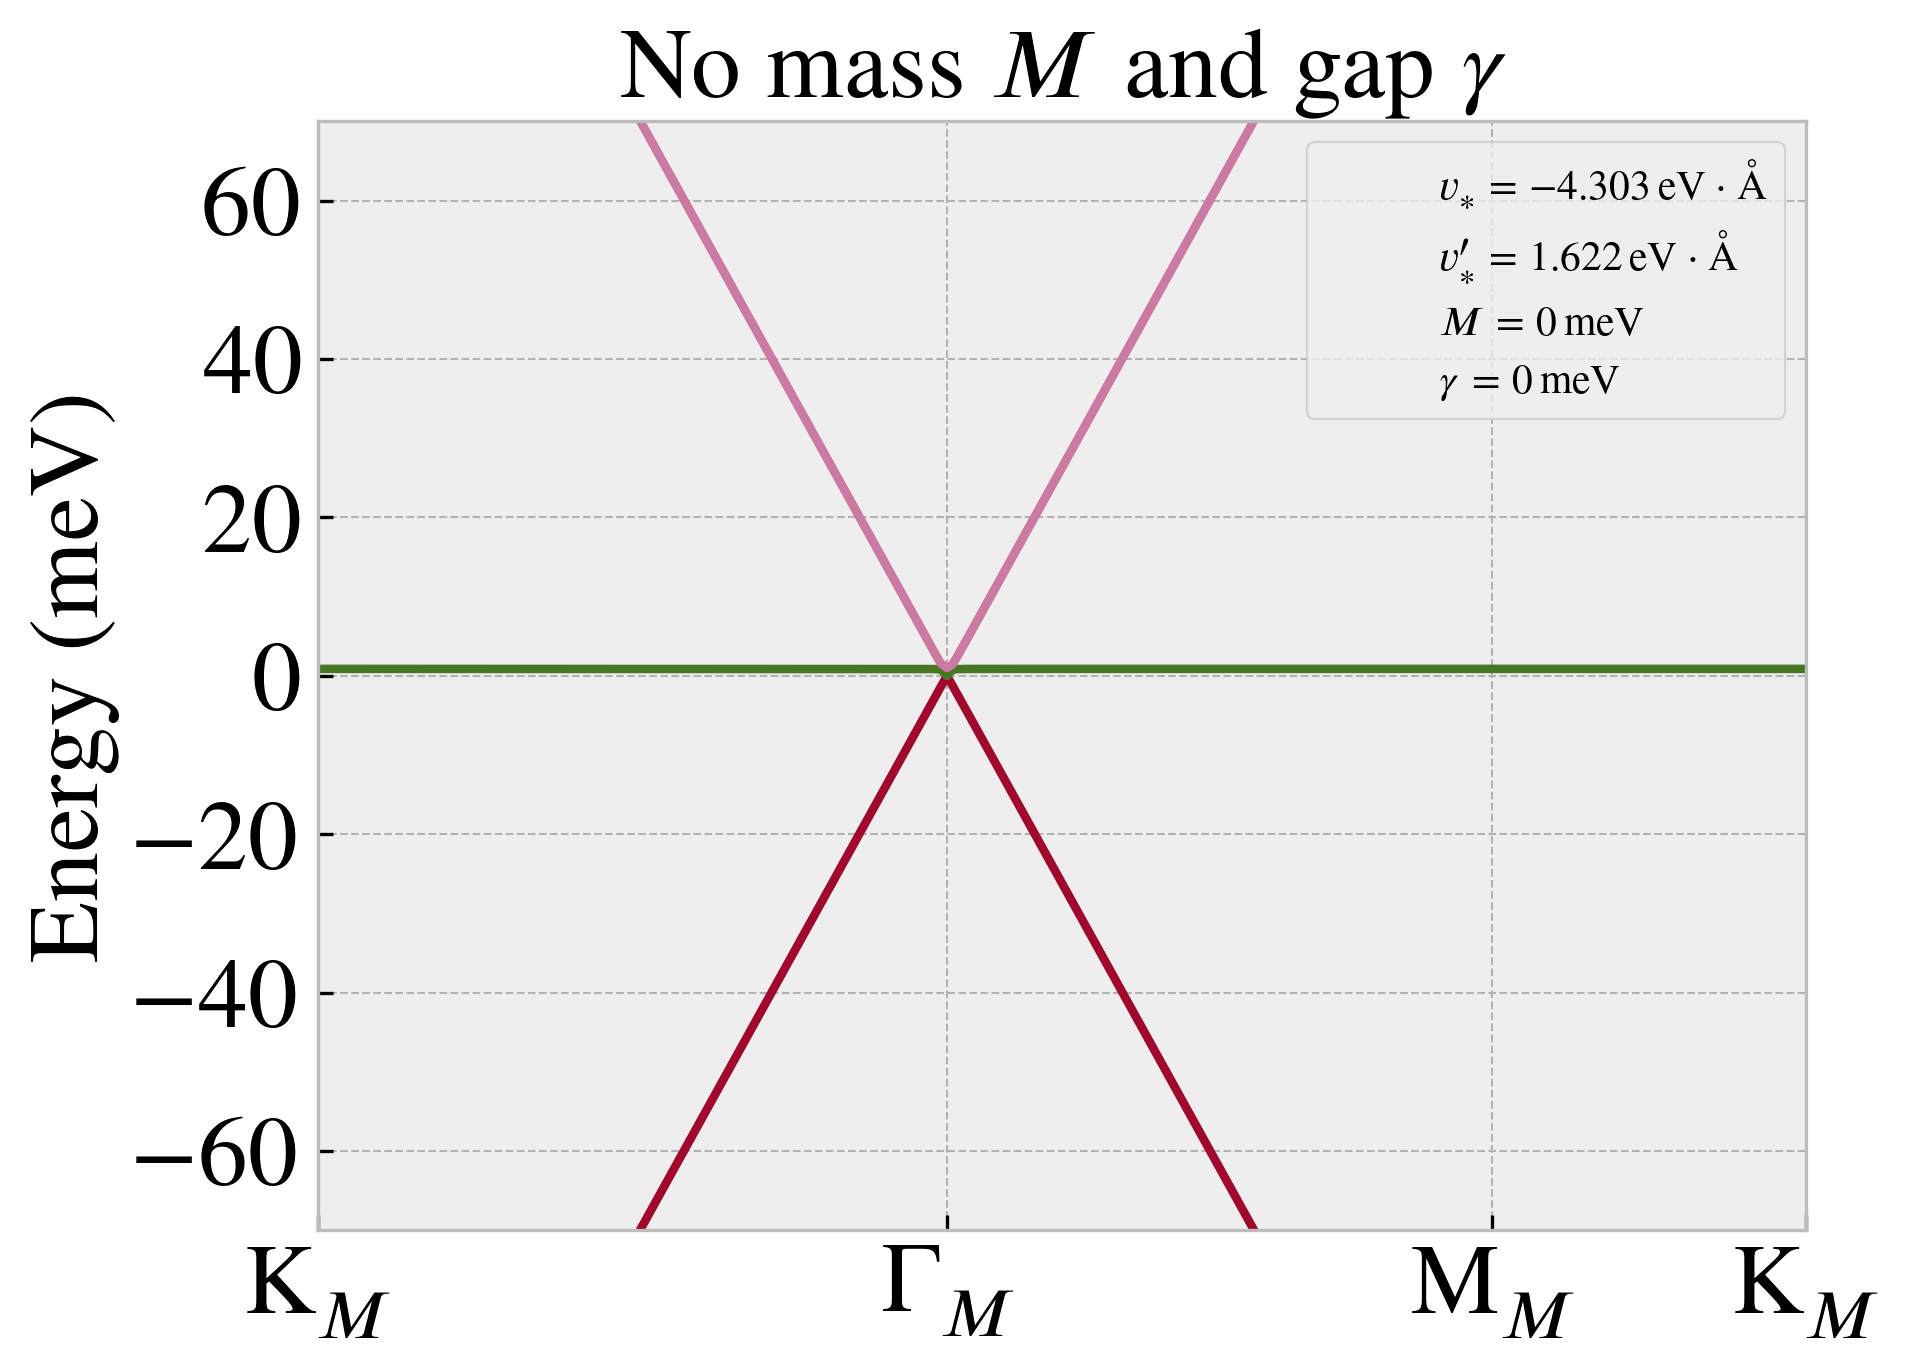
\includegraphics[height=0.25\linewidth]{fig/thf-no_M_no_gamma.png}
%%%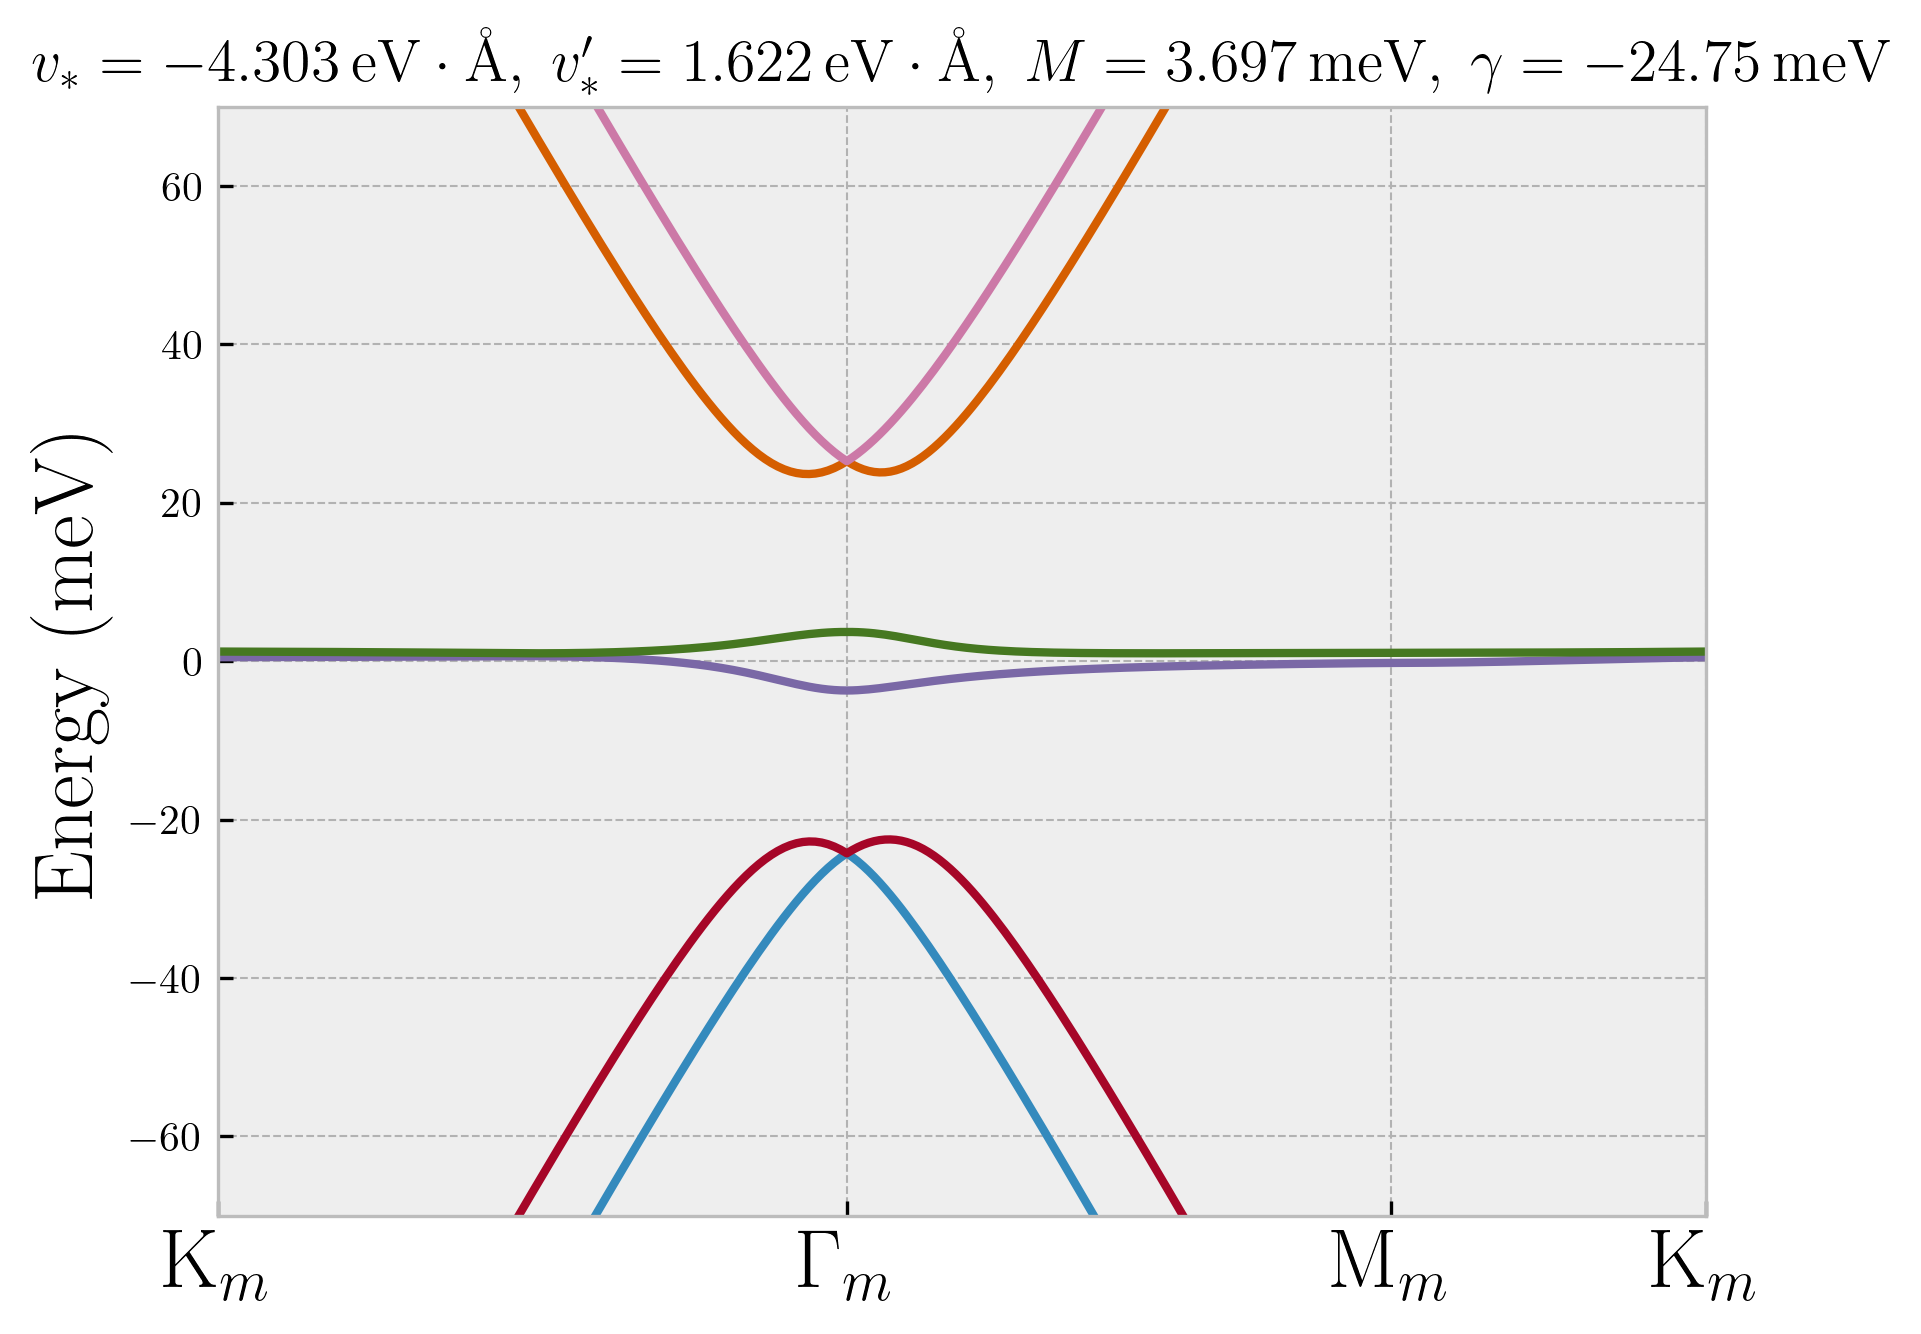
\includegraphics[height=0.35\linewidth]{fig/thf-correct_params.png}
%%%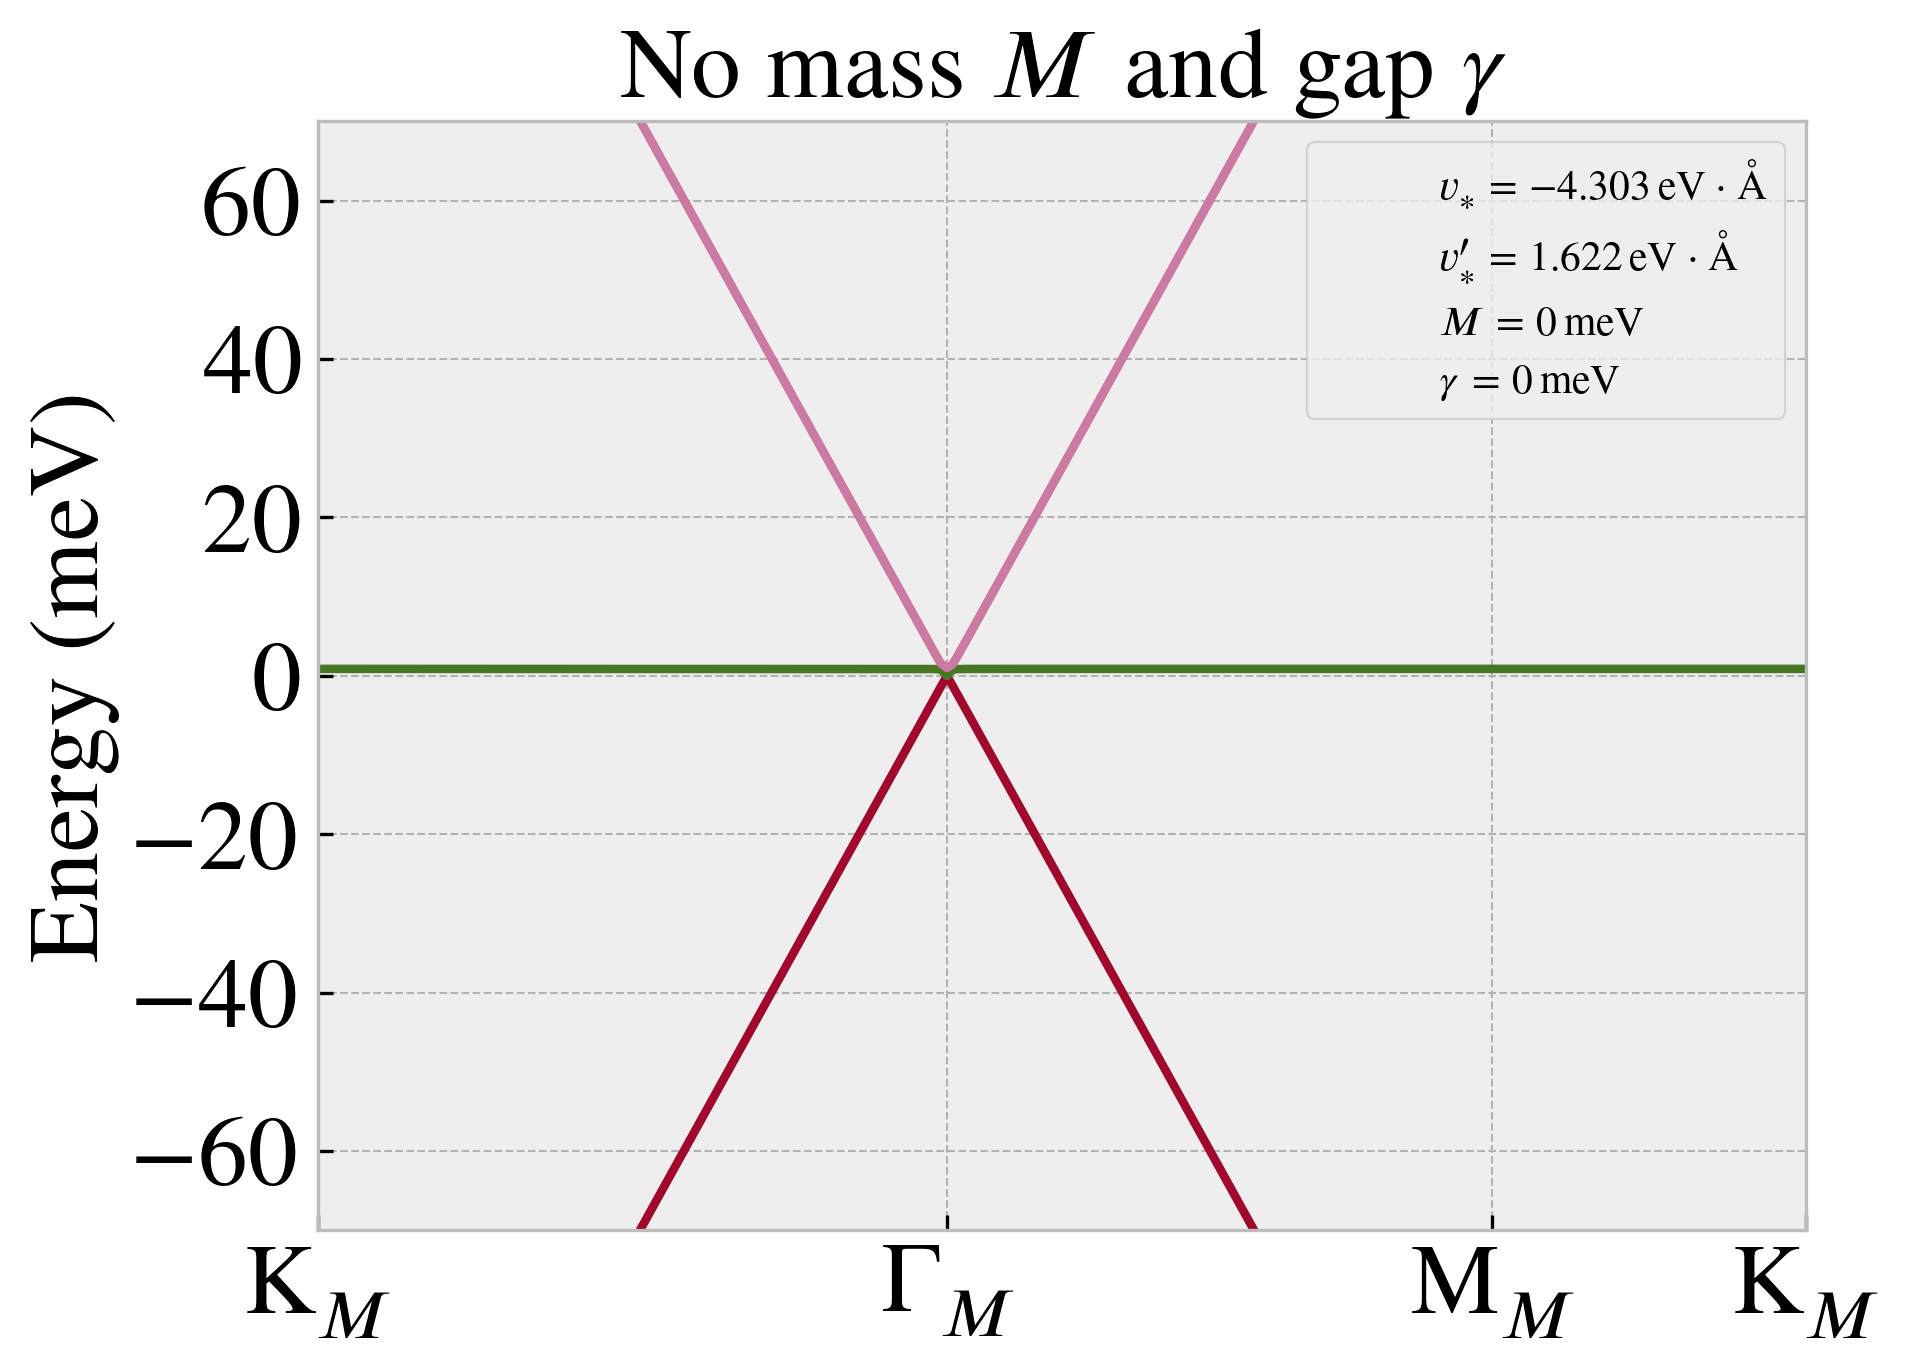
\includegraphics[height=0.35\linewidth]{fig/thf-no_M_no_gamma.png}
%%\caption{}
%\label{fig:thf-correct_params}
%\end{figure}
%\begin{figure}[H]
%\centering
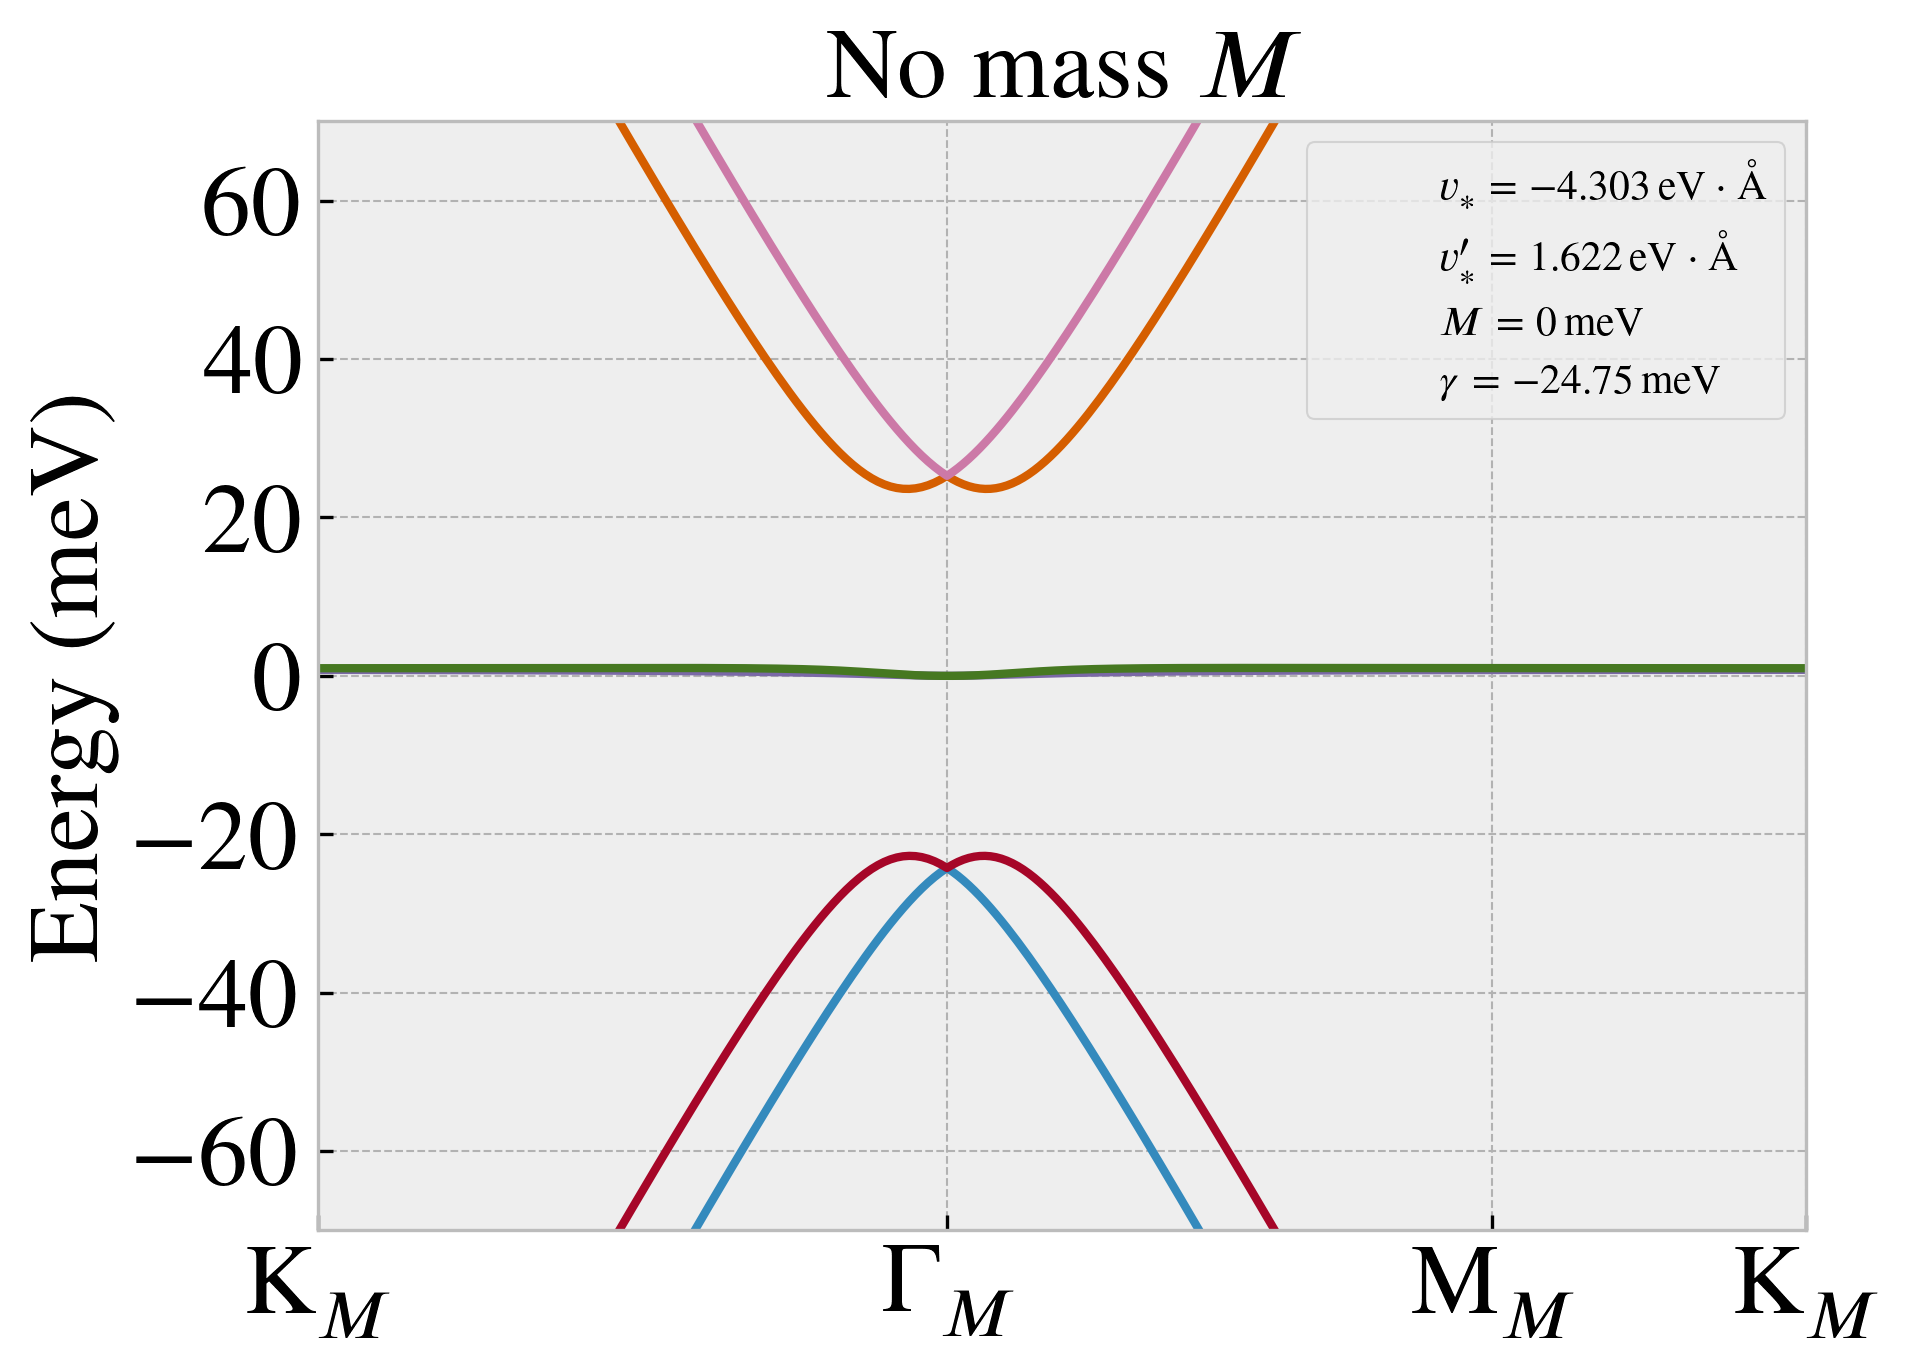
\includegraphics[height=0.25\linewidth]{fig/thf-no_M.png}
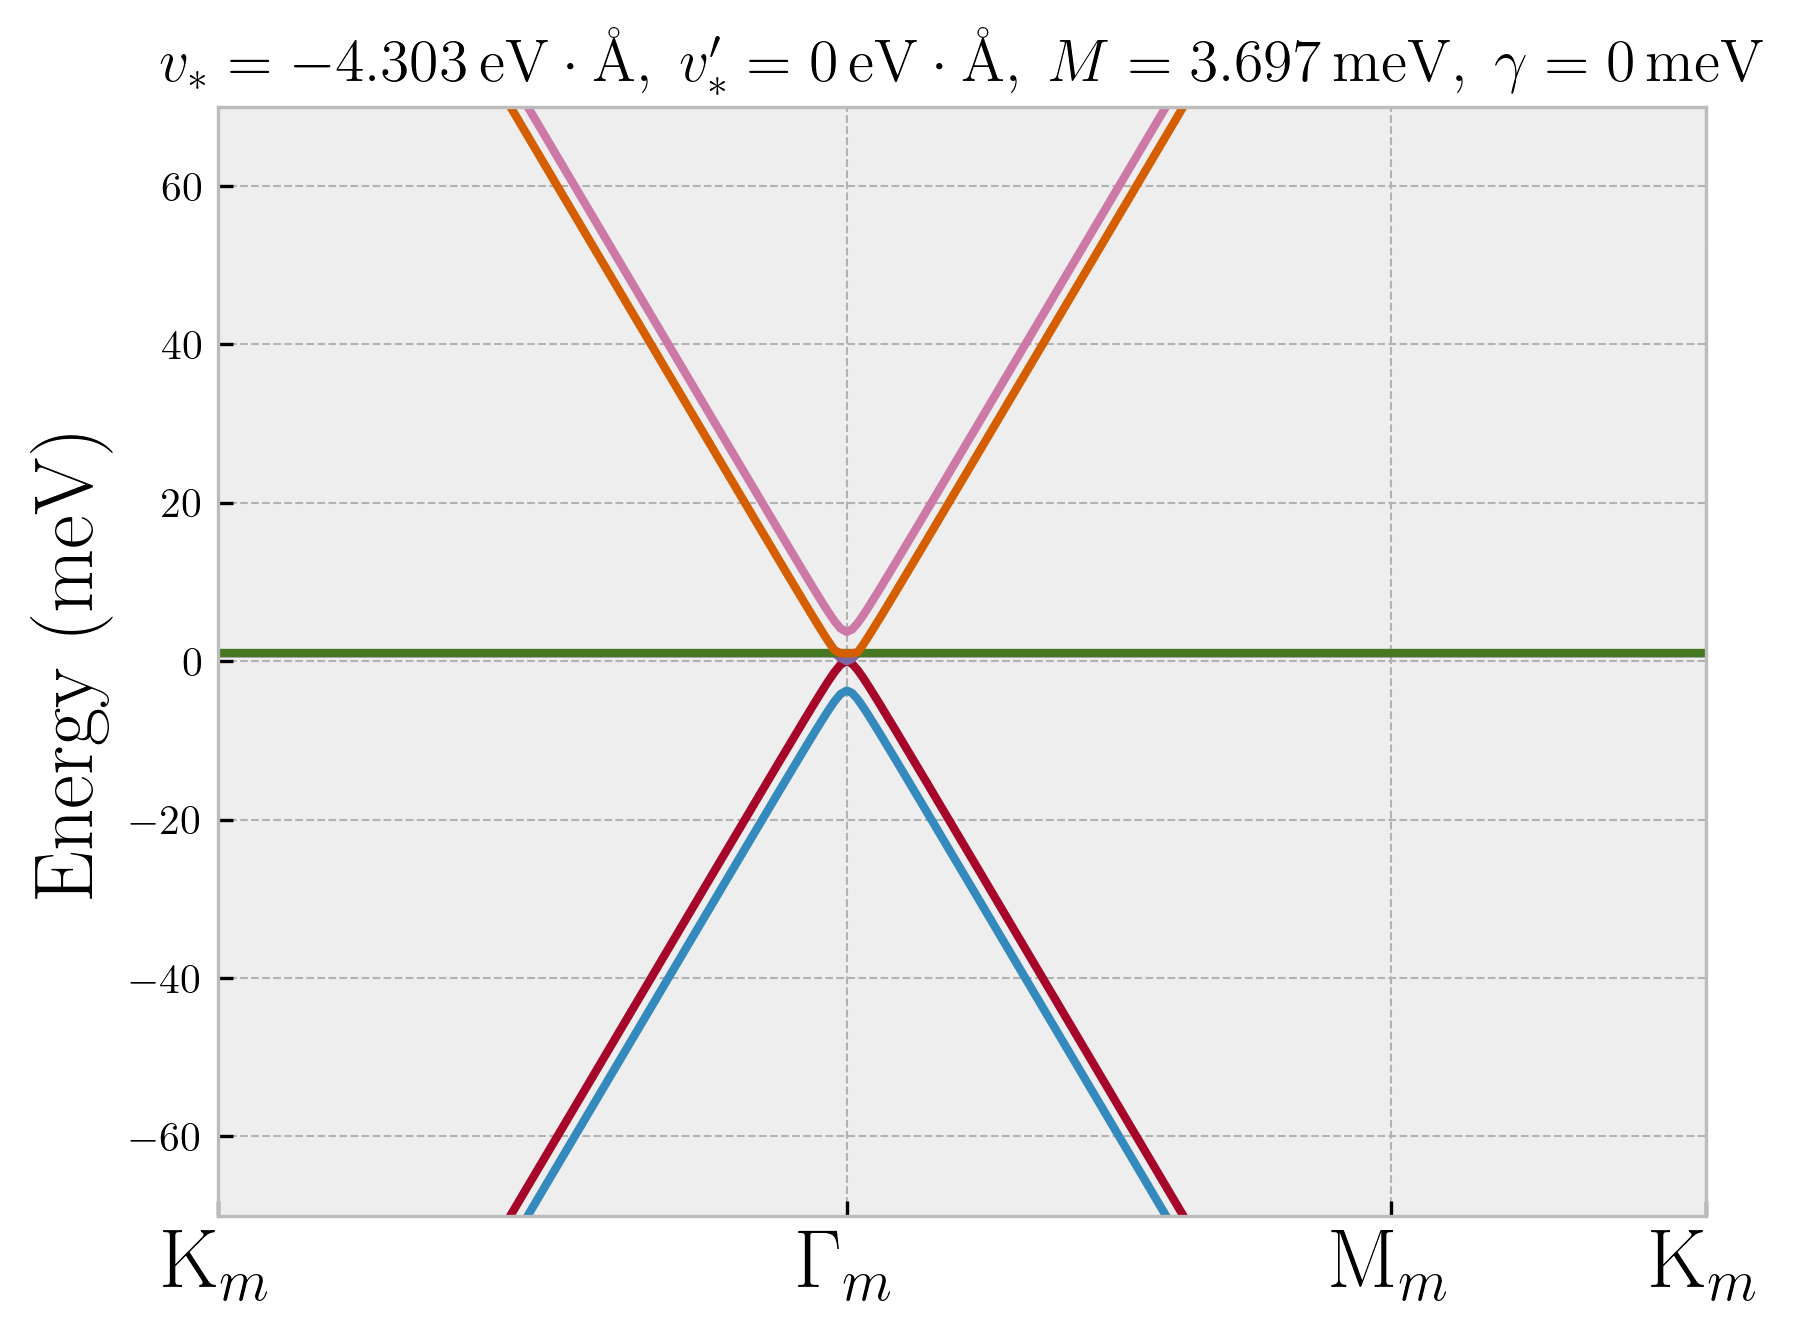
\includegraphics[height=0.25\linewidth]{fig/thf-no_coupling.png}
%%%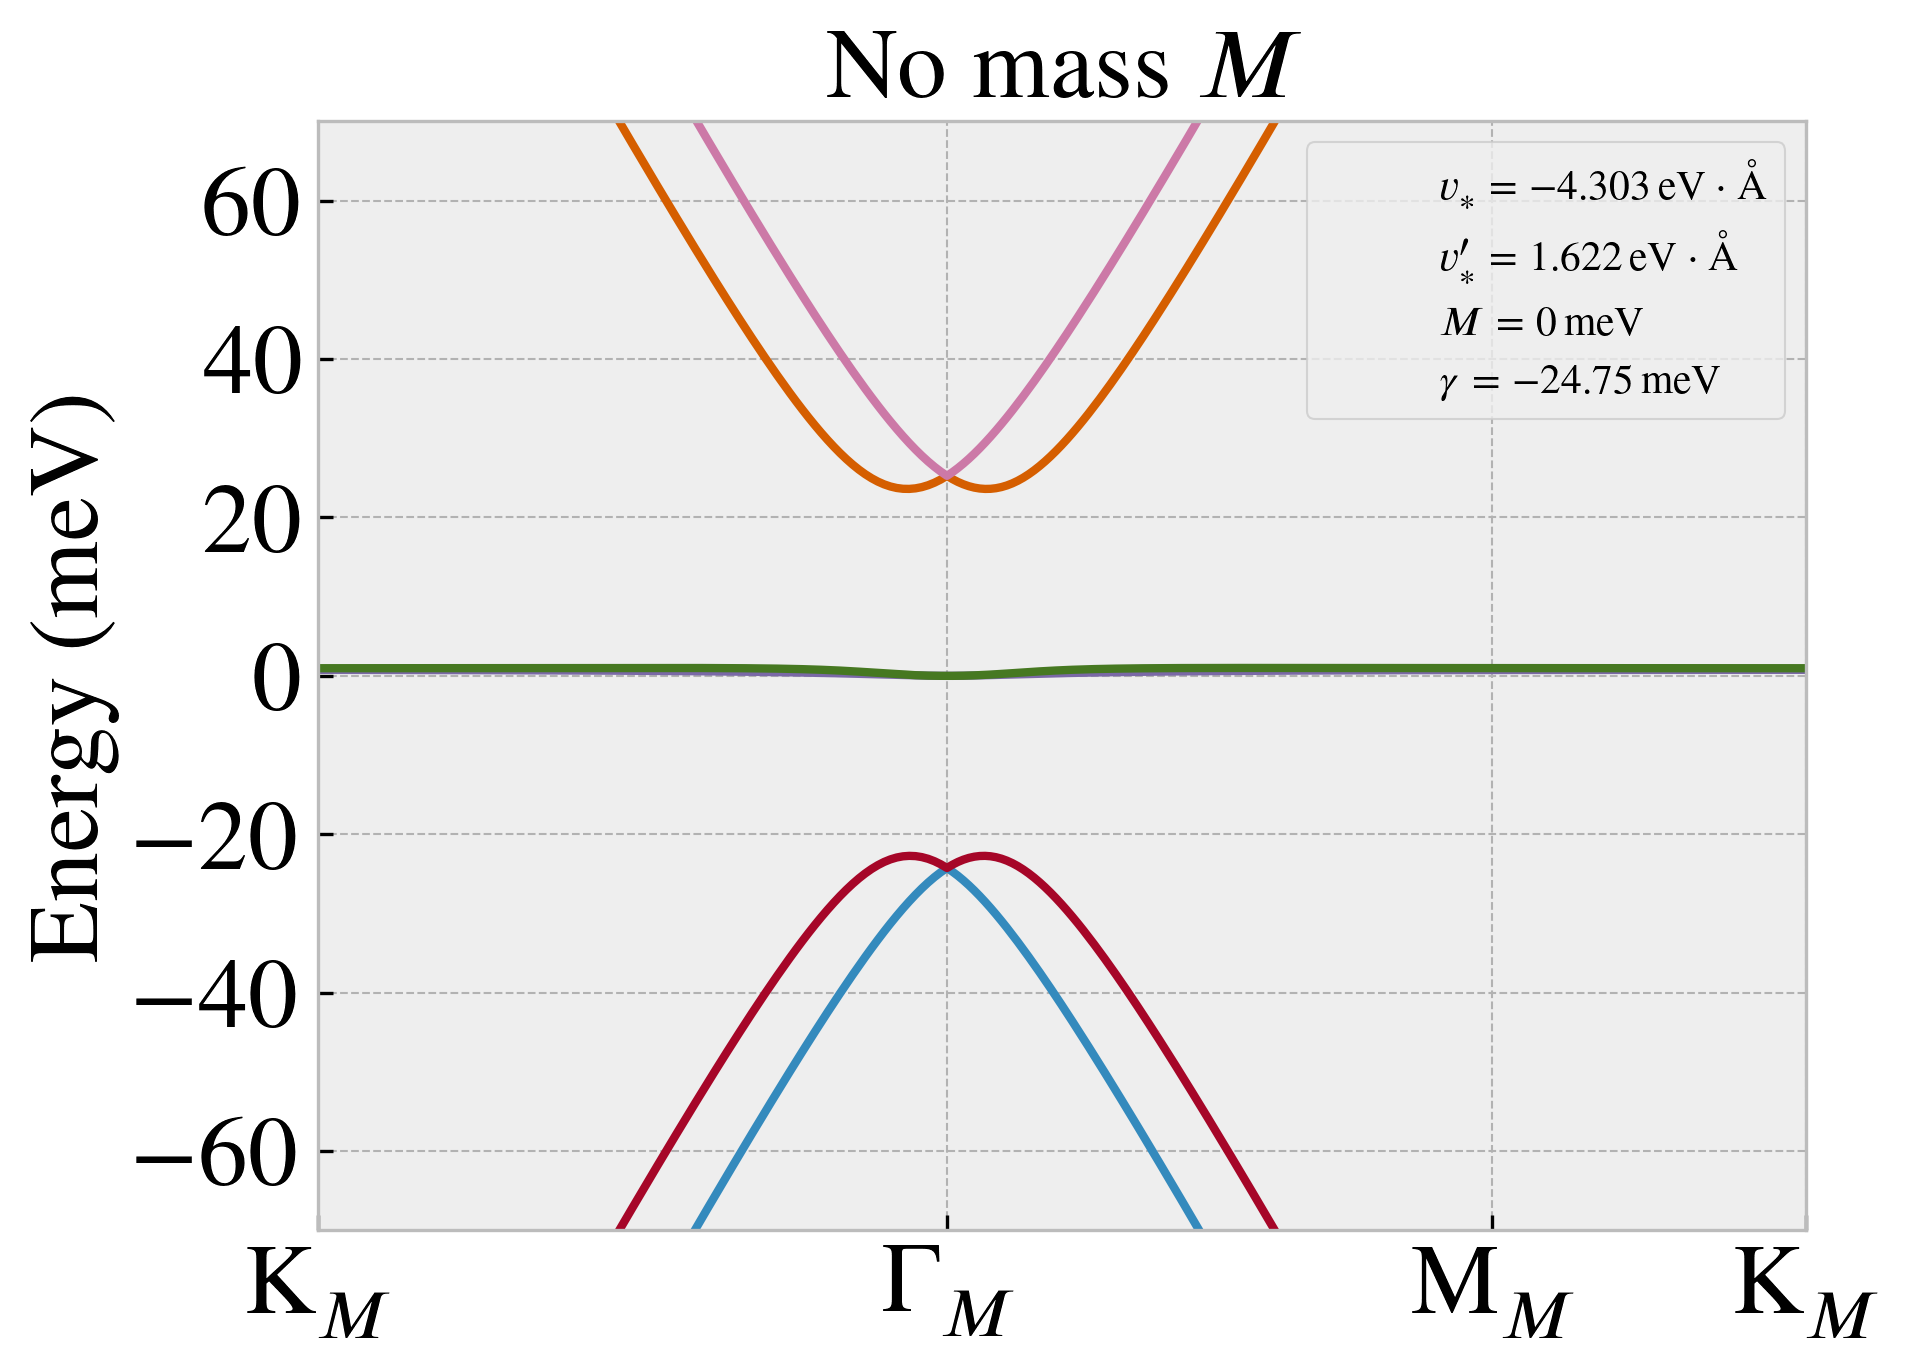
\includegraphics[height=0.35\linewidth]{fig/thf-no_M.png}
%%%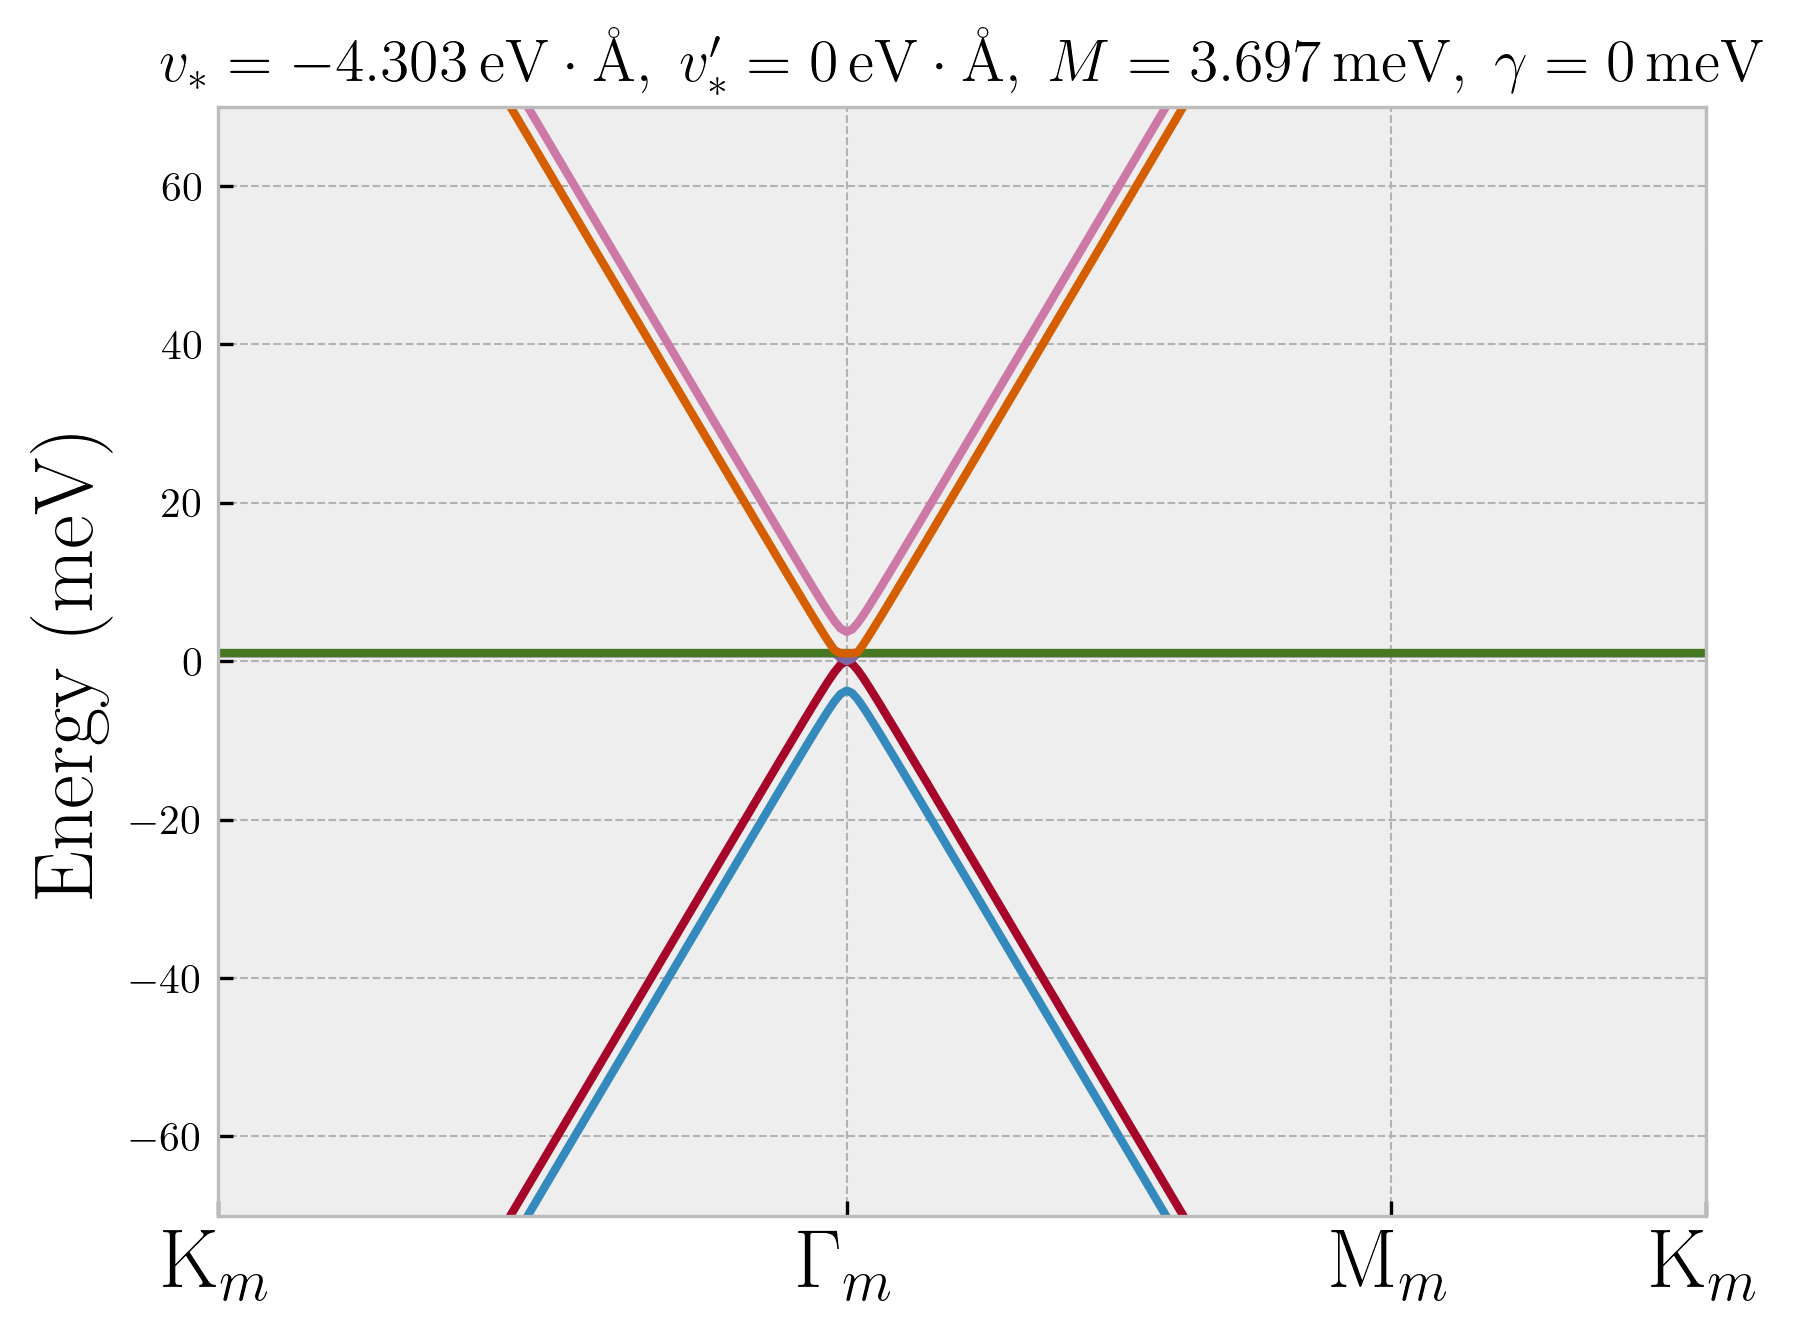
\includegraphics[height=0.35\linewidth]{fig/thf-no_coupling.png}
\caption{Band structures for the 6-band non-interacting Topological Heavy Fermion model, showing the effect of different parameters on the electronic states. Each panel illustrates a variation of the model with certain parameters set to zero.}
\label{fig:thf-exploration}
\end{figure}




%%%%%%%%%%%%%%%%%%%%%%%%%%%%%%%%%%%%%%%%%%%%%%%%%%%%%%%%%%%%%%%%%%%%%%%%%%%%%%%%%%%%%%%%%%%%%%%%%%
%%%%%%%%%%%%%%%%%%%%%%%%%%%%%%%%%%%%%%%%%%%%%%%%%%%%%%%%%%%%%%%%%%%%%%%%%%%%%%%%%%%%%%%%%%%%%%%%%%


%%%%%%%%%%%%%%%%%%%%%%%%%%%%%%%% COMMENT THIS TO COMPILE main.tex %%%%%%%%%%%%%%%%%%%%%%%%%%%%%%%%
%%%-----
%%% Referências bibliográficas
%%%-----
%\addcontentsline{toc}{chapter}{\bibname}
%%\bibliographystyle{abntex2-num}
%\bibliography{citations}
%\bibliographystyle{ieeetr}
%\end{document}
%%%%%%%%%%%%%%%%%%%%%%%%%%%%%%%% COMMENT THIS TO COMPILE main.tex %%%%%%%%%%%%%%%%%%%%%%%%%%%%%%%%
